% chapters/chapter4.tex  — converted from chapter4.typ
% Conventions used (identical to chapter1.tex / chapter2.tex / chapter3.tex):
%   Typst @KEY            -> \ac{KEY}            (auto: long on first use, short after)
%   Typst @KEY:lo         -> \acl{KEY}          (long form only)
%   Typst @figlabel       -> Figure~\ref{fig:figlabel}
%   Typst @tablabel       -> Table~\ref{tab:tablabel}
%   Typst @sec_label      -> Section~\ref{sec:label}
%   Typst @chN            -> Chapter~\ref{chN}
%   Typst @eqt:eq_label   -> Equation~\eqref{eq:label}
%   Typst @citekey        -> \cite{citekey}
%   Typst `code`          -> \texttt{code}      (underscores and & escaped)
%   Typst _italic_        -> \emph{italic}
%   Typst "quoted"        -> \enquote{quoted}
% The Typst `#import "functions.typ"` has no LaTeX counterpart and is dropped.
%
% NOTE: cross-refs resolve against labels defined in chapter3.tex
%       (sec:sysid, sec:vision, eq:lane_shift, tab:arch_summary) and against
%       \label{ch2}, \label{ch3}. They are all present in the converted chapters.

\chapter{Simulation Results and Evaluation}
\label{ch4}

The previous chapter developed three lateral-control architectures for the \ac{LKA} function and motivated each design choice on control-theoretic grounds. The present chapter complements that theoretical discussion with the numerical evaluation of the three controllers in CARLA. All experiments are run on the same test route in Town06, with the same vehicle (\texttt{vehicle.nissan.patrol}), the same target speed of $30$~km/h, the same simulation rate $T_s = 0.05$~s, and the same set of PID gains obtained from the system-identification procedure of Section~\ref{sec:sysid}. Under these conditions, any observed difference between the trajectories can be attributed to the structure of the error signal and to the corresponding controller rather than to incidental variations in the simulator.

The chapter is structured as follows. Section~\ref{sec:exp_setup} describes the experimental protocol, the reference path and the metrics used to compare the controllers. Section~\ref{sec:carla_view} presents a qualitative view of the test route as rendered inside the CARLA world. Section~\ref{sec:full_traj} quantifies the tracking performance over the entire route. Section~\ref{sec:smooth_turn} and Section~\ref{sec:lane_change} then zoom in on two representative sections of the route---the long smooth curve and a sudden lane discontinuity---where the differences between the three architectures become most visible. Section~\ref{sec:discussion} finally interprets the results in the light of the control-theoretic predictions of Chapter~\ref{ch3}.

\section{Experimental Setup}
\label{sec:exp_setup}
The reference path was recorded once, in autopilot mode, by driving the ego vehicle through Town06 and logging the closest waypoint at every simulation tick, as described in Chapter~\ref{ch2}. The resulting \texttt{carla\_data.csv} file contains a strictly monotonic sampling of the center line along an approximately $L$-shaped route of about $850$~m. The route starts on a north--south urban street, executes a $90^\circ$ left turn onto a long east--west arterial, and ends after a stretch of straight road that includes a step-like lane discontinuity---a feature that proves particularly informative when comparing the three controllers. The route was selected because it exercises both the steady-state behavior of the controllers, on the long straight section that follows the turn, and their transient behavior, on the corner itself and on the lane discontinuity.

Three closed-loop experiments were then performed on this same route, one for each architecture:

\begin{itemize}
    \item \emph{Cross-track PID} (\texttt{lane\_shift\_pid/pygame\_controller.py}). The reference is the recorded path; the error is the cross-track distance Equation~\eqref{eq:lane_shift}; the controller is a full PID with the gains $K_p, K_i, K_d$ produced by \texttt{pid\_tuning.py} for $\omega_n^{\mathrm{lat}} = 1.5$~rad/s. The trajectory is logged to \texttt{ego\_trajectory\_shift.csv} and appears in blue on every plot of this chapter.
    \item \emph{Heading-error PI} (\texttt{heading\_error\_pid/pygame\_controller.py}). The reference is again the recorded path, but the error is the look-ahead heading angle; the controller is a PI with the gains produced by \texttt{pid\_tuning.py} for $\omega_n^{\mathrm{lat}} = 2.0$~rad/s. The trajectory is logged to \texttt{ego\_trajectory\_heading.csv} and appears in green.
    \item \emph{Vision-based PI} (\texttt{detection\&pid.py}). The reference is reconstructed at every tick from the RGB camera by the CLRNet lane detector~\cite{clrnet} followed by the \acs{IPM} projection of Section~\ref{sec:vision}. The same PI controller of the previous architecture consumes the heading error computed in the body frame. At intersections the \ac{LKA} hands off to the CARLA Traffic Manager autopilot, as described in Section~\ref{sec:vision}. The trajectory is logged to \texttt{ego\_trajectory\_vision.csv} and appears in red.
\end{itemize}

The longitudinal channel is identical in the three experiments: a discrete PI regulator drives the speed to $30$~km/h with the gains obtained from the longitudinal step experiment of Section~\ref{sec:sysid}. All three trajectories are post-processed by \texttt{plot\_trajectory.py}, which overlays the recorded reference path and computes two scalar performance metrics:

\begin{itemize}
    \item The \emph{\acl{RMSE}}, \ac{RMSE} $e_y = \sqrt{(1/N) \sum_{k=1}^N e_y[k]^2}$, which summarizes the average tracking accuracy over the run;
    \item The \emph{maximum absolute cross-track error}, $\max \lvert e_y \rvert = \max_{k} \lvert e_y[k] \rvert$, which captures the worst-case excursion from the center of the lane.
\end{itemize}

For the vision-based run, the cross-track error reported by the plotting script is computed \emph{a posteriori} against the same recorded reference path used by the other two runs, even though the controller itself never has access to that path. This makes the three runs comparable on a common metric and isolates the effect of the perception layer from the rest of the control loop. It is also worth stressing that the cross-track error used here as a comparison metric is \emph{not} the error signal of the heading-error and vision-based controllers: those two controllers close their loop on an angle, and the cross-track distance is only computed \emph{off-line} for evaluation purposes.

\section{Qualitative View in CARLA}
\label{sec:carla_view}
Before turning to the numerical metrics, it is useful to look at the test route as it appears in the simulator itself. The script \texttt{draw\_trajectory\_in\_carla.py} takes a logged trajectory and draws it as a coloured line directly in the CARLA world, on top of the textured road, using the simulator's debug-drawing API. The start of the trajectory is marked with a green sphere and the end with a red sphere. Figure~\ref{fig:traj_carla} reproduces one of these renderings for the heading-error PI run, which is the controller that achieves the best tracking accuracy over the full route.

\begin{figure}[htbp]
    \centering
    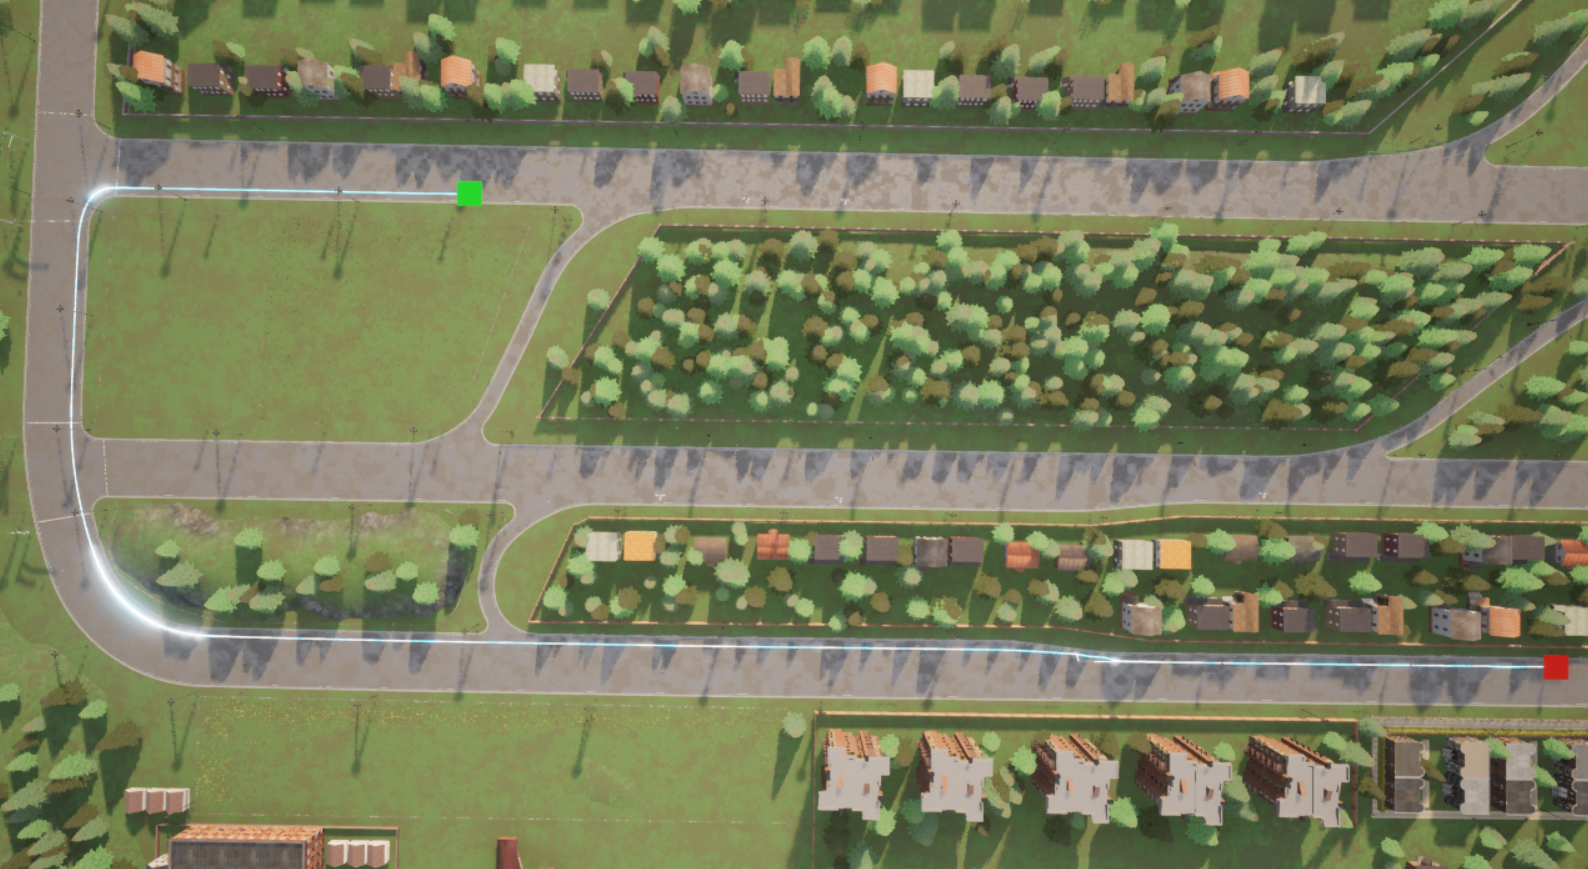
\includegraphics[width=0.8\linewidth]{image/fig_trajectory_in_carla.png}
    \caption{Top-down view of Town06 with the trajectory of the heading-error PI controller drawn in cyan by \texttt{draw\_trajectory\_in\_carla.py}. The green square marks the start of the run, the red square marks the end. The vehicle enters from the top of the figure, executes a $90^\circ$ left turn at the intersection, and proceeds east along the arterial. The line stays well inside the lane throughout the manoeuvre, which is the basic visual confirmation that the controller fulfils its \acs{LKA} purpose. The remaining discussion of this chapter focuses on the quantitative differences between the three architectures along this same route.}
    \label{fig:traj_carla}
\end{figure}

Two observations can already be made from the in-simulator view. First, the trajectory stays well inside the lane throughout the manoeuvre---the rendered line never leaves the asphalt and remains close to the center of the lane on both the curved and the straight sections of the route. This is the minimum requirement for a \ac{LKA} and the most basic safety check. Second, the corner itself is the most demanding part of the route: it concentrates a large change in the reference heading into a short stretch of road and produces the largest transients in the cross-track error, as the next section will show.

\section{Full-Route Tracking Performance}
\label{sec:full_traj}
The first quantitative comparison is performed over the entire route. Figure~\ref{fig:traj_full} shows the top-down trajectory plot (left) and the cross-track error as a function of time (right), with the three controllers overlaid on the same axes and with the \ac{RMSE} and maximum absolute error reported in the legend.

\begin{figure}[htbp]
    \centering
    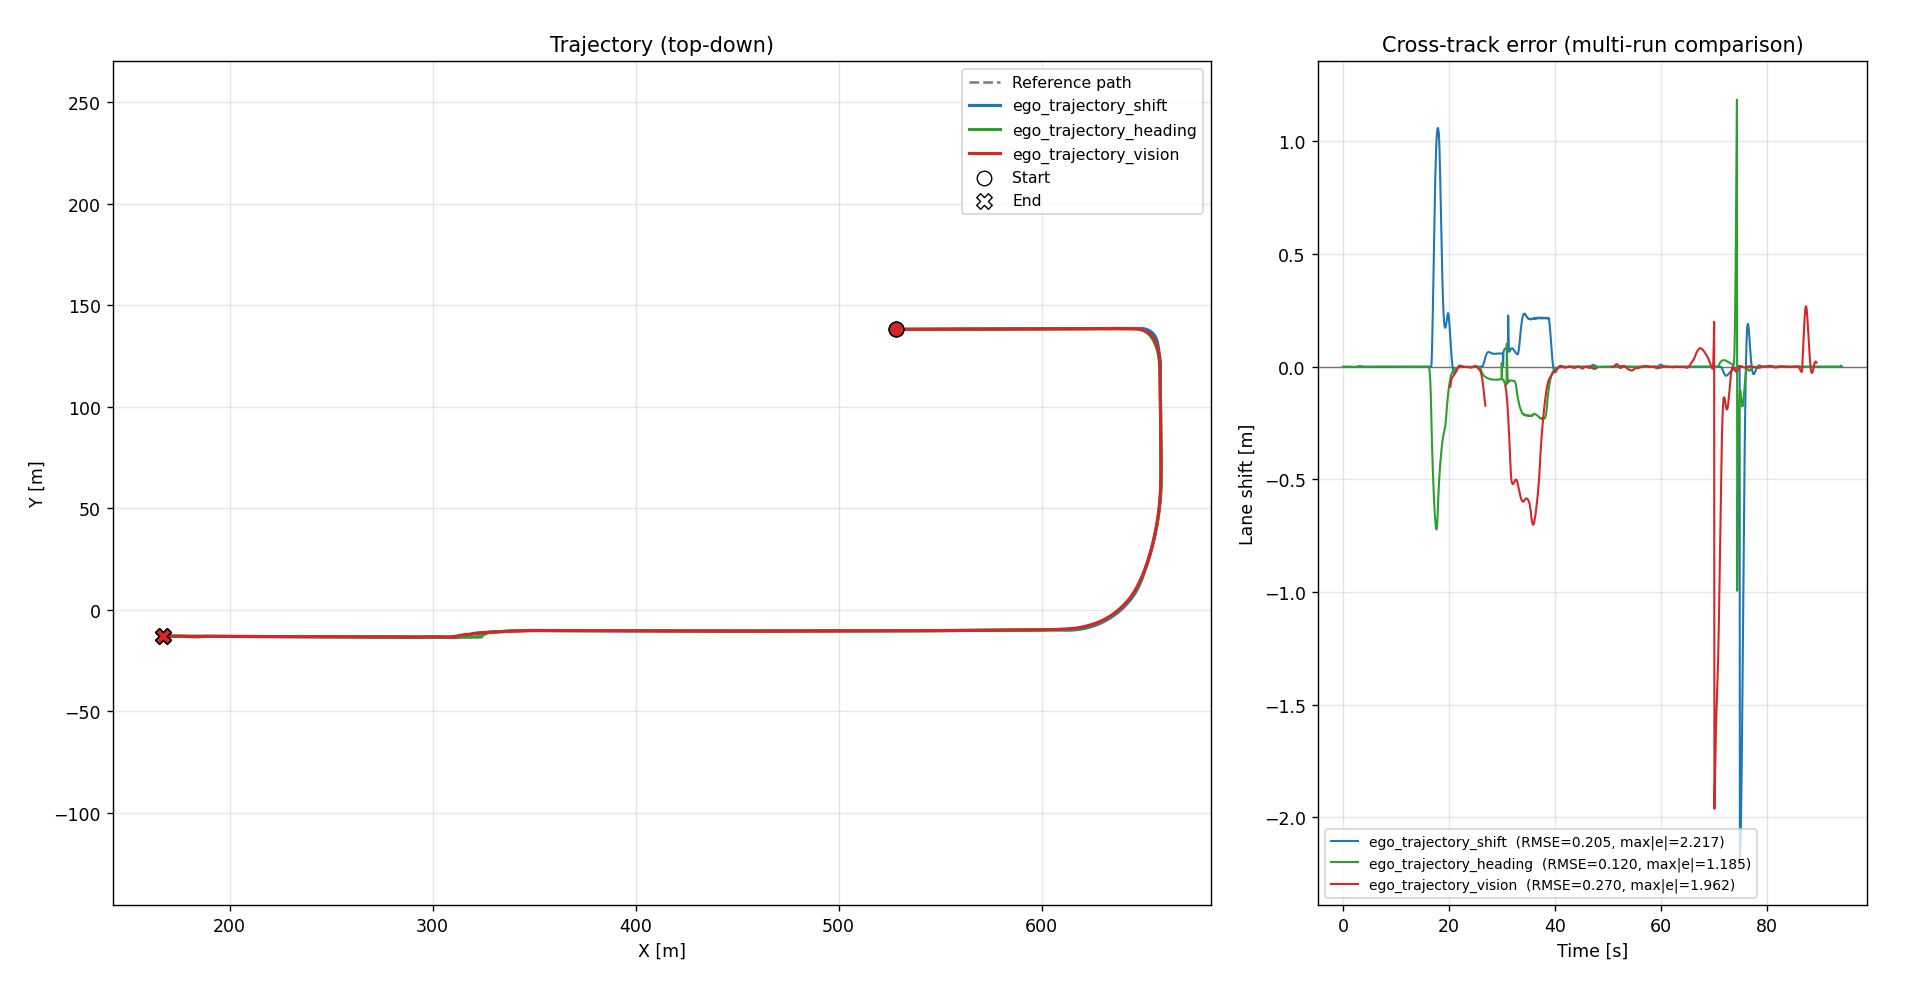
\includegraphics[width=\linewidth]{image/fig_trajectory_full.png}
    \caption{Full-route comparison of the three controllers. \emph{Left}: top-down view of the recorded reference path (grey dashed) and of the three closed-loop trajectories (cross-track PID in blue, heading-error PI in green, vision-based PI in red). Start and end of each run are marked with circles and crosses respectively. \emph{Right}: cross-track error $e_y(t)$ as a function of time, with the root-mean-square error and the maximum absolute error reported in the legend. The two large transients around $t \approx 18$--$22$~s and $t \approx 70$--$75$~s correspond respectively to the $90^\circ$ corner and to a step-like lane discontinuity in the reference path.}
    \label{fig:traj_full}
\end{figure}

A few comments on the figure. On the long straight section that follows the corner---roughly from $t \approx 25$~s to $t \approx 60$~s---the three trajectories are visually indistinguishable from the reference at the scale of the left-hand panel, even though small but persistent biases are visible on the right-hand error trace. These steady-state biases are the subject of Section~\ref{sec:smooth_turn}. The two large excursions occur at the $90^\circ$ corner, where the cross-track and the vision-based controllers overshoot by approximately $1$~m, and at the step-like lane discontinuity around $t \approx 70$--$75$~s, where the maximum excursions of the run are recorded. Note that the cross-track error trace of the vision-based controller has a finite duration: the controller starts logging only once the lane detector returns a valid center line, which is the reason why the red curve is missing on the very first seconds of the trace.

The numerical metrics extracted from the right-hand panel are summarized in Table~\ref{tab:full_metrics}. The heading-error PI achieves both the lowest \ac{RMSE} and the lowest maximum excursion of the three architectures, by a clear margin. The cross-track PID is intermediate in \ac{RMSE} but exhibits the worst maximum excursion of the three runs at the lane discontinuity. The vision-based PI has the highest \ac{RMSE}, mainly because of a persistent steady-state bias on the smooth curve that the next section will analyze in detail.

\begin{table}[htbp]
    \centering
    \footnotesize
    \begin{tabular}{@{} l c c l @{}}
        \toprule
        \textbf{Controller} & \textbf{\acs{RMSE} $e_y$ [m]} & \textbf{$\max \lvert e_y \rvert$ [m]} & \textbf{Worst-case event} \\
        \midrule
        Cross-track PID  & $0.205$ & $2.217$ & Step-like lane discontinuity \\
        \addlinespace
        Heading-error PI & $0.120$ & $1.185$ & Step-like lane discontinuity \\
        \addlinespace
        Vision-based PI  & $0.270$ & $1.962$ & Step-like lane discontinuity \\
        \bottomrule
    \end{tabular}
    \caption{Tracking metrics over the entire route, read directly from the legend of Figure~\ref{fig:traj_full}. Lower is better.}
    \label{tab:full_metrics}
\end{table}

The relative ordering of the three controllers---heading-error best, cross-track intermediate, vision-based worst on \ac{RMSE}---matches the qualitative prediction of Table~\ref{tab:arch_summary} on the structural argument (heading-error preferred over cross-track because of the lower plant order) but adds a new piece of information that the theoretical chapter could not anticipate: the perception layer of the vision-based controller introduces a steady-state bias on the smooth curve that dominates its \ac{RMSE}. The maximum-excursion ordering is different: there, the worst performer is the cross-track PID at $2.22$~m, with the vision-based PI at $1.96$~m and the heading-error PI at $1.19$~m. All three peaks coincide in time with the step-like lane discontinuity of the reference path, which is a deliberately adversarial test case discussed in Section~\ref{sec:lane_change}.

\section{Performance on a Smooth Curve}
\label{sec:smooth_turn}
The first zoom-in focuses on the long smooth curve that occurs after the corner, between $t \approx 25$~s and $t \approx 45$~s. The road curvature in this section is gentle and approximately constant, so the relevant figure of merit is the \emph{steady-state cross-track error} that each controller maintains while tracking a constant-curvature reference. Figure~\ref{fig:traj_smooth} shows the top-down trajectory (left) and the cross-track error (right) restricted to this section of the route.

Three quantitative observations can be made from Figure~\ref{fig:traj_smooth}. The cross-track PID (blue) settles to a positive steady-state error of approximately $+0.22$~m, which means that the vehicle rides on the \emph{outside} of the curve relative to the center line. This is the classical signature of a PID that is fighting a constant disturbance---the road curvature acts as a constant input to the lateral plant---and that has not yet had the time to absorb it through its integral term. The heading-error PI (green) settles to a negative steady-state error of approximately $-0.22$~m, which means that the vehicle rides on the \emph{inside} of the curve. The opposite sign of the two biases is a direct consequence of the different error signal: the cross-track controller tries to keep $e_y = 0$ at the closest waypoint, whereas the heading-error controller tries to keep the look-ahead angle $\alpha = 0$, and the look-ahead point on a curved reference is geometrically inside the curve relative to the closest waypoint. The two biases have similar magnitude but they reflect two different geometric definitions of \enquote{being on the center}.

\begin{figure}[H]
    \centering
    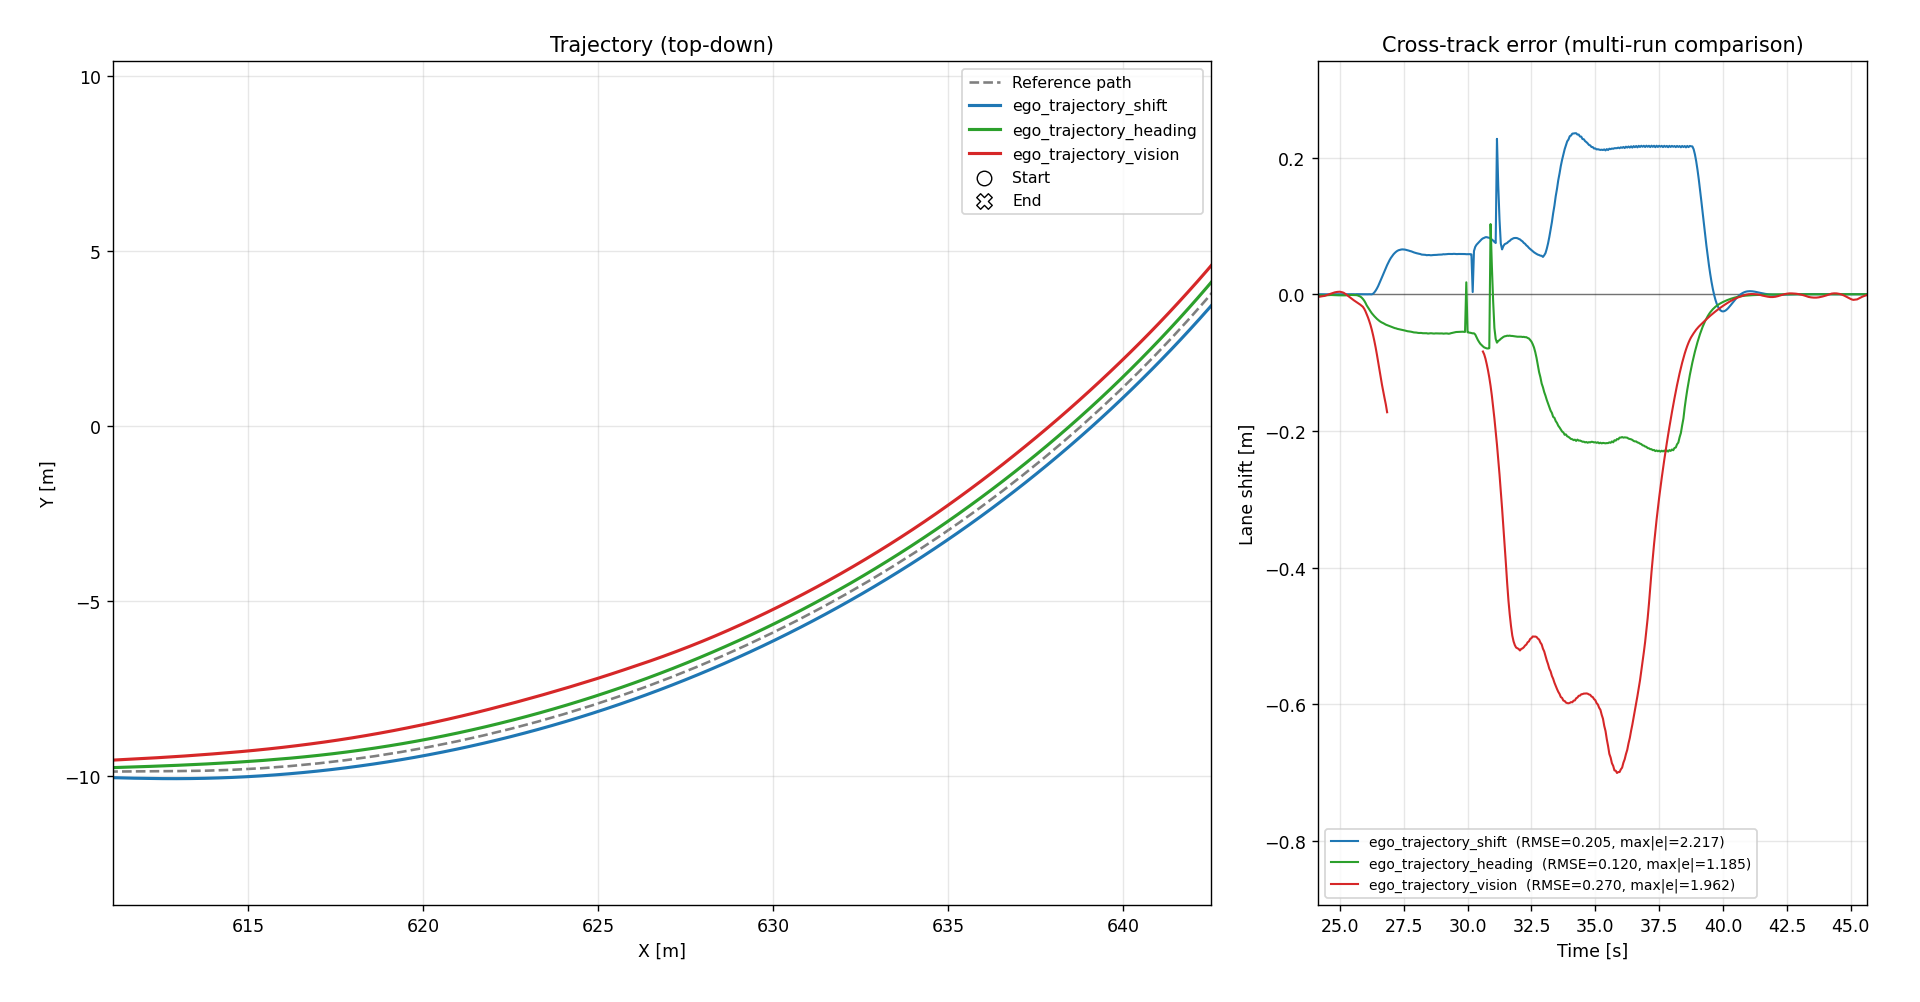
\includegraphics[width=\linewidth]{image/fig_trajectory_smooth_turn.png}
    \caption{Smooth-curve detail. \emph{Left}: top-down view of the recorded reference (grey dashed) and of the three closed-loop trajectories along a gentle, approximately constant-curvature stretch of road between $X \approx 615$~m and $X \approx 640$~m. The three controllers track the same curve with different signed steady-state biases that are clearly visible at this magnification. \emph{Right}: corresponding cross-track error between $t \approx 25$~s and $t \approx 45$~s. The vision-based PI exhibits a large negative bias that reaches $\approx -0.7$~m at the apex of the curve, while the cross-track PID and the heading-error PI settle to biases of opposite sign with comparable magnitude of $\approx +0.22$~m and $\approx -0.22$~m respectively.}
    \label{fig:traj_smooth}
\end{figure}

The vision-based PI (red) exhibits a much larger negative bias that reaches approximately $-0.7$~m at the apex of the curve, a factor of three larger than the heading-error PI on which it is built. The two controllers share the same control law and the same gains; the only difference is the source of the look-ahead point. The conclusion is that the additional bias is introduced by the perception layer. Two mechanisms contribute to it. First, the center line returned by \texttt{get\_centerline} is the average of the two \emph{detected} lane boundaries, which are themselves curved; the mid-point of two parallel arcs is biased toward the inside of the curve by an amount proportional to the curvature and to the lateral spacing between the boundaries. Second, the first-degree polynomial fit of Section~\ref{sec:vision} approximates a locally curved center line with a straight line, which systematically truncates the lateral component of the look-ahead target. Both mechanisms have the same sign and combine into the observed bias. On a straight road, neither mechanism is active and the vision-based controller behaves exactly like the heading-error PI, which is consistent with the near-zero error reported in Figure~\ref{fig:traj_full} before $t \approx 25$~s.

It is also worth noting that the magnitudes involved here---$0.22$~m for the path-based controllers and $0.7$~m for the vision-based controller---remain comfortably within the half-width of a typical CARLA lane, which is approximately $1.75$~m. The biases on the smooth curve therefore do not threaten the safety of the \ac{LKA} function; they only degrade the comfort and the tracking accuracy.

\section{Performance on a Sudden Lane Discontinuity}
\label{sec:lane_change}

\begin{figure}[H]
    \centering
    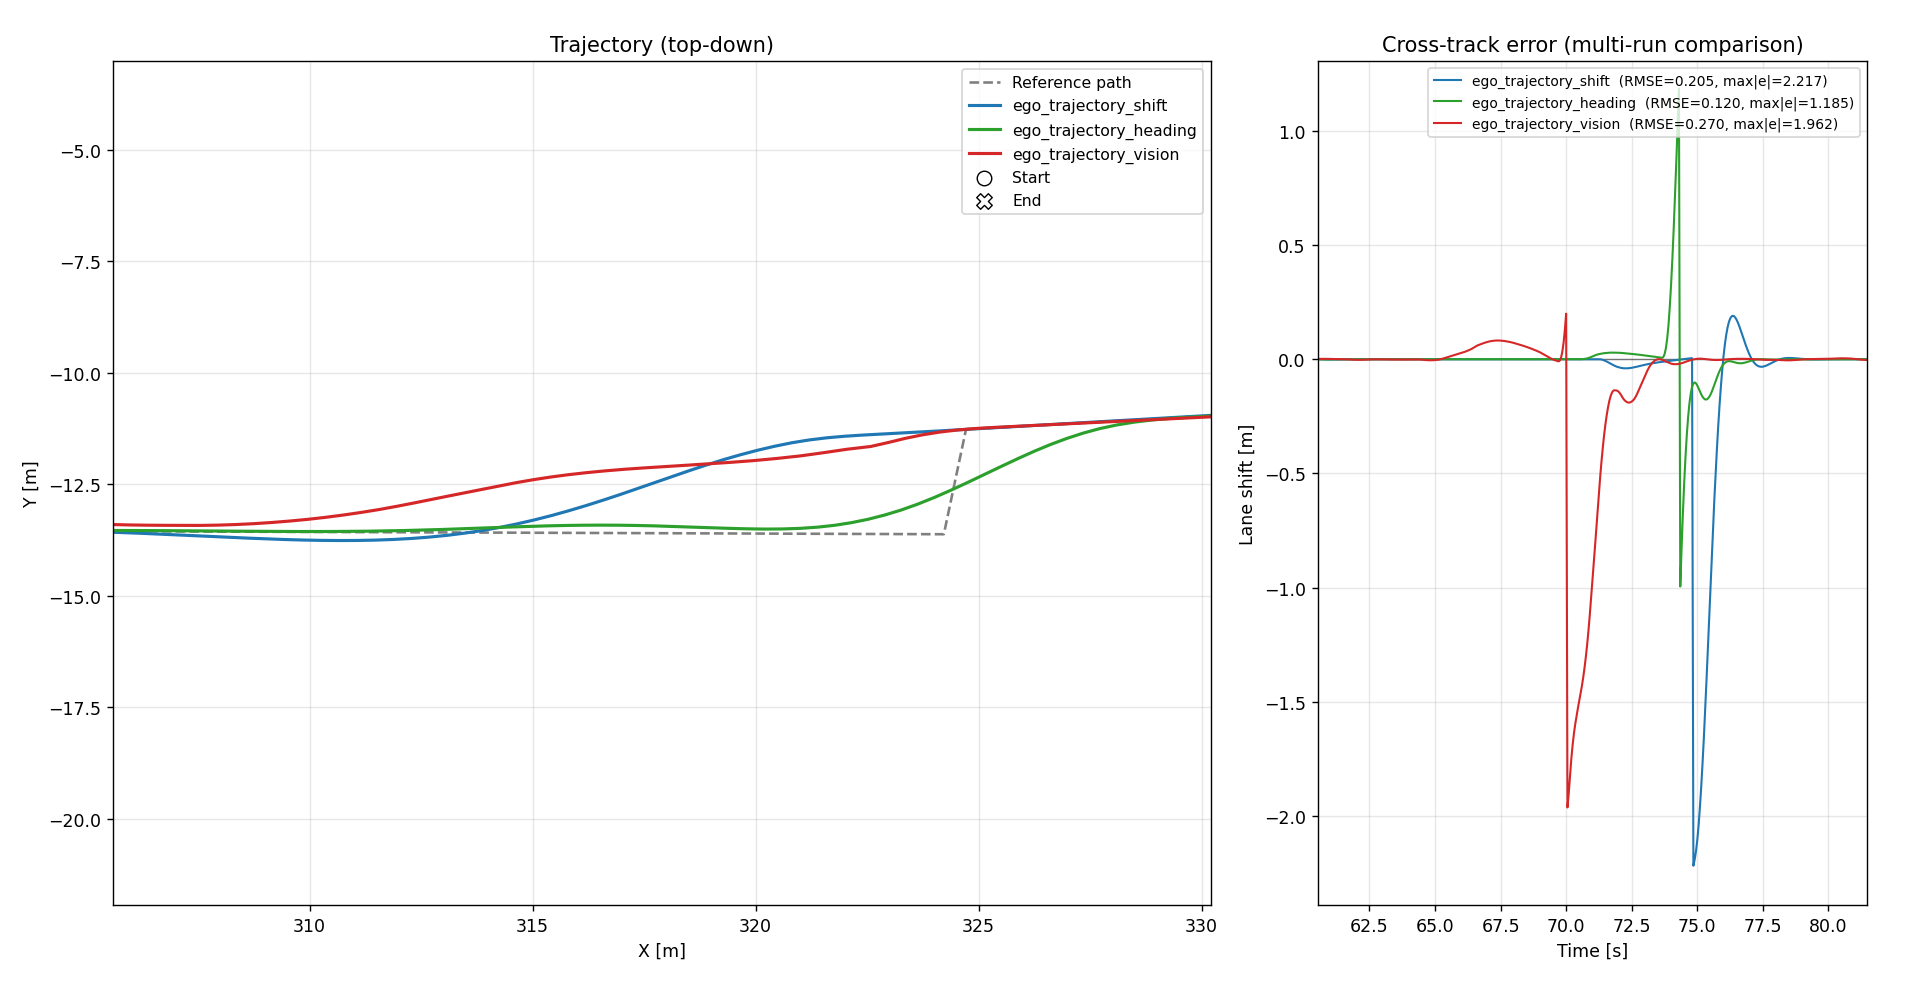
\includegraphics[width=0.85\linewidth]{image/fig_trajectory_lane_change.png}
    \caption{Step-like lane discontinuity. \emph{Left}: top-down view of the reference (grey dashed) and of the three closed-loop trajectories in the neighborhood of the discontinuity. The reference exhibits a step of approximately $3$~m at $X \approx 325$~m. The three controllers react with very different transients. \emph{Right}: cross-track error between $t \approx 60$~s and $t \approx 80$~s. The cross-track PID (blue) takes the largest excursion at $\approx -2.22$~m; the vision-based PI (red) anticipates the discontinuity and undershoots by $\approx -1.96$~m around $t \approx 70$~s; the heading-error PI (green) is the smoothest of the three, with a single overshoot of $\approx +1$~m.}
    \label{fig:traj_change}
\end{figure}

The second zoom-in focuses on a step-like discontinuity of the reference path that occurs around $t \approx 70$--$75$~s, which corresponds to the right-hand spikes visible in Figure~\ref{fig:traj_full} and which is shown in detail in Figure~\ref{fig:traj_change}. This discontinuity is an artefact of the way the reference path was recorded: when the vehicle in autopilot mode merged from one lane into an adjacent one, the closest-waypoint logger jumped from the center line of the first lane to the center line of the second one, which produces a step of approximately one lane width ($3$~m) in the reference. From the controller's point of view, this is the worst possible kind of disturbance: a step in the reference rather than a step in the disturbance input.

The three controllers react to the step in three qualitatively different ways. The cross-track PID (blue) follows the original lane up to the discontinuity, then suddenly sees a large positive cross-track error appear on its closest waypoint and reacts with a large steering input that overshoots the new lane by $\approx 2.2$~m on the opposite side. This is the worst-case event of the whole run for this controller, and it is the manifestation of the limited phase margin of the cross-track loop: a step on the input of a double integrator is integrated twice before the controller has any chance to react, and the resulting overshoot is bounded only by the rate-limited saturation of the steering actuator. The transient takes approximately $2$~s to decay.

The heading-error PI (green) reacts differently. The look-ahead point is, by construction, several meters ahead of the vehicle; the controller therefore \enquote{sees} the discontinuity coming and starts steering toward the new lane before the discontinuity is reached. The cross-track error in Figure~\ref{fig:traj_change} shows a much smaller positive transient of approximately $+1$~m, followed by a small undershoot of $-1$~m as the look-ahead point crosses the step in the opposite direction. The transient is over within a single look-ahead time horizon, that is in less than $1$~s. The maximum-excursion metric on this controller is the smallest of the three at $1.19$~m, which is essentially this single peak.

The vision-based PI (red) reacts earliest of all three because the lane detector reconstructs the upcoming center line several meters ahead of the vehicle and the polynomial fit smooths the discontinuity into a gradual lateral shift. The cross-track error trace shows a large negative excursion that starts at $t \approx 67$~s---well before the path-based controllers react---and reaches $\approx -2$~m at $t \approx 70$~s. This is \emph{not} a tracking failure: the vehicle is correctly following what the camera sees, and what the camera sees is a smooth lateral shift rather than a step. The error is large because the metric is computed against the path-based reference, which itself contains the step. In a real-world deployment, where the only reference is the camera image, this trajectory would actually be the smoothest and the most natural-feeling of the three.

The lane-discontinuity event therefore illustrates the fundamental difference between the three approaches: the path-based controllers track a pre-recorded reference and are penalized by any discontinuity in that reference, while the vision-based controller tracks what is actually painted on the road and can naturally absorb such discontinuities at the cost of an inevitable lag with respect to a discontinuous ground-truth metric.

\section{Discussion}
\label{sec:discussion}
The numerical results of this chapter both confirm and refine the control-theoretic predictions of Chapter~\ref{ch3}. The reduction of one plant integrator from the cross-track to the heading-error formulation buys a measurable improvement in tracking accuracy: the heading-error PI achieves an \ac{RMSE} of $0.120$~m against the $0.205$~m of the cross-track PID, a factor of $1.7$ improvement, and a maximum excursion of $1.19$~m against $2.22$~m, a factor of $1.9$ improvement. Both numbers are consistent with the larger phase margin and the gentler gain schedule that Table~\ref{tab:arch_summary} attributed to the heading-error formulation.

The addition of a perception layer on top of the heading-error PI is less clear-cut. On a straight road, the vision-based controller is indistinguishable from its path-based counterpart, as expected. On a smooth curve, the perception layer introduces a steady-state bias of approximately $-0.7$~m that the controller cannot remove because it never sees the path-based reference. This bias is the price to pay for being independent of a pre-recorded map. On a step-like lane discontinuity, the perception layer is actually beneficial because it smooths the discontinuity into a gradual lateral shift; the large excursion that appears on the cross-track error metric is an artefact of the comparison against a discontinuous reference, not a tracking failure of the controller.

A subtler point is the role of the controller speed of reaction. The heading-error PI uses a look-ahead distance of $L_d \approx 9$~m at $30$~km/h, which gives the controller approximately $1$~s of preview on the reference. The vision-based PI uses the same preview horizon but applies it to a perception-based reference. The cross-track PID has no preview at all: it reacts to the closest waypoint, which is by definition the present, not the future. The factor of $1.9$ on the maximum excursion between the cross-track and the heading-error controllers is therefore not only a consequence of the lower plant order, but also of the implicit feed-forward that the look-ahead introduces. Disentangling the two effects would require an additional experiment in which the cross-track PID is augmented with an explicit feed-forward term computed from the road curvature; this is left for future work.

From a practical standpoint, the experiments support the following recommendations for an \ac{LKA} function deployed in this kind of simulation environment. The cross-track PID is the simplest of the three architectures to implement and tune, but it is the most sensitive to discontinuities in the reference and to changes in the vehicle speed; it is acceptable for low-speed, smooth-path applications. The heading-error PI is the most accurate and the most robust to reference discontinuities; it is the recommended choice whenever a pre-recorded reference path is available. The vision-based PI is the only one of the three that does not depend on a pre-recorded map; it pays for this independence with a steady-state bias on curves, which can be mitigated either by a higher-order polynomial fit of the center line or by a curvature-aware correction of the look-ahead point. The detailed implementation of these mitigations is the subject of the chapter on future work.

The next chapter draws the overall conclusions of the thesis and outlines the directions for future investigation.
